% EPC flow charts
% Author: Fabian Schuh
\documentclass{article}
\usepackage{myflowchart}

\begin{document}
\begin{tikzpicture}
\begin{scope}[node distance=5mm and 5mm]

\node [ item=2](a) at (1,1) {%
            \textbf{未完成方向}
            \nodepart[text width = 8.2cm]{two}
            \begin{enumerate}
            	\item 應用subdoc讓case\_g20.tex及其他可以獨立運行,就不用去擔心編譯時期相對路徑找不到檔問題。
            	\item share community, tikz, LYX doc, ...
            	\item Math.lyx與.pdf清楚化$\bullet\bullet\bullet\circ$
            	\item LYX做webpost時的標題列css模組化$\bullet\circ\circ\circ$,目前是用python做代換。
            	\item sciencefair typeset conti, 將疊格繪圖方程modulize.
           \end{enumerate}
            };

\node [ wideitem=2, above right = of a, anchor = south](incentive) {%
            \textbf{incentive}
            \nodepart{two}An auxiliary unit of TeX service providing typeset specialty to the website group and to the gyro simulation group. This unit also provides customized TeX service to other business.
            };

\node [above = of incentive, align = center] (title){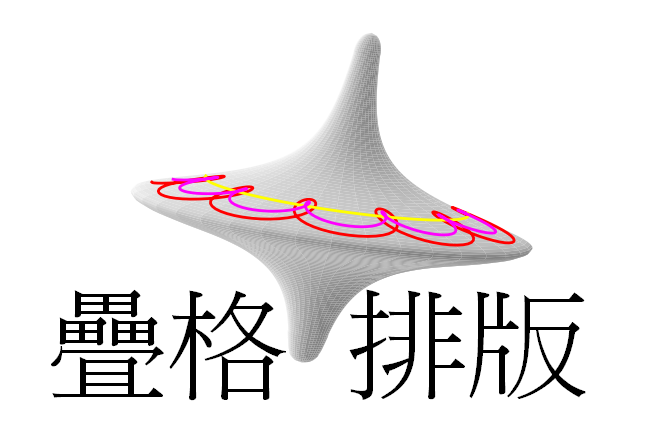
\includegraphics[width=0.4\textwidth]{../../figs/tex_logo.png}\\ \LARGE 事業部規劃};


\node [ item=2, below right = of incentive.south, anchor = north west](unique) {%
            \textbf{特色}
            \nodepart[text width = 8.2cm]{two}
            \begin{enumerate}
            	\item 使用LYX與SW,高度自動化(省下很多細微瑣碎步驟)。
            	\item 與不同應用做方便性整合,如django,web blog等等。
           \end{enumerate}
            };

\node [ item=2,below = of a](small) {%
            \textbf{還需思考的未完成項目}
            \nodepart[text width = 8.2cm]{two}
            \begin{enumerate}
		\item LYX mailing list post suggestion on align environment. Check dev group on this.
		\item LYX export包含有被伺服圖檔的html檔,目前已有一寫下的流程,但還是要做成自動化較方便。
            	\item vec A不對稱問題?
            	\item 順著陀螺外型的powered by LYX SW字串,path?
		\item texlive 2017 installed, but texworks fails to start?! dwmapi.dll找不到。instead using gvim now.
	    \end{enumerate}
            };

\node [ item=2,below = of small](direct) {%
            \textbf{可直接進行的未完成項目}
            \nodepart[text width = 8.2cm]{two}
            \begin{enumerate}
		\item 畫openGL coordinate圖並加說明。
            	\item 加入tikz說明書,node position,anchor參數必須要在above right之類參數之後才會有效。去github fork先report issue,然後加說明書?
	    \end{enumerate}
            };
\node [ item=2, below = of unique](LYXcustomization) {%
            \textbf{LYX特殊客製化紀錄}
            \nodepart[text width = 8.2cm]{two}
            \begin{enumerate}
            	\item 在LYX中直接加入ScriBD的pdf preview視窗指令,LYX export html後即可成為一具有Scribd pdf預覽視窗的網頁。範例請見網站的疊格服務介紹網頁。
           	\begin{enumerate}
           		\item 步驟:使用LYX的program listing指令,在指令中貼上Scribd的embed pdf指令,存檔。使用LYX的export html指令,我有新增一複製指令,所以html檔除了存在原本檔案位置,也會存到django的template資料夾。去template夾中,打開LYX2HTML\_str\_replace.py檔,確認fname是該html檔名,關閉py檔。執行python LYX2HTML\_str\_replace.py檔。
           	\end{enumerate}
           \end{enumerate}
            };

\node [ item=2, below = of LYXcustomization](SWcustomization) {%
            \textbf{SW特殊客製化紀錄}
            \nodepart[text width = 8.2cm]{two}
            \begin{enumerate}
            	\item 在SW中若要加入連結,由於SW本身的inserted hypertext所插入的msihyperref指令在xelatex下編譯會多產生兩個??,因此只好用平常的hyperref指令,並且這樣的話也可以很方便的把連結加顏色換型變得很漂亮。不過這樣的話以後要輸入就要去複製一個平常的hyperref指令,然後更改其中的連結成想要的。是有點麻煩,之後再想辦法。
           \end{enumerate}
            };


\end{scope}
\end{tikzpicture}

%Second page
\begin{tikzpicture}
\begin{scope}[node distance=5mm and 5mm]

\node [ item=2](gitlog) at (1,1) {%
            \textbf{last 10 git commits}
            \nodepart[text width = 8.2cm]{two}
            \footnotesize \verbatiminput{xelatex.log}
            };

\end{scope}
\end{tikzpicture}


\end{document}
